% CHAPTER 3: Self attention
\chapter{Self-Attention}

Consider the sentence: \textit{”The animal didn't cross the street because it was too tired”}. What does the word "it" refer to? For a human, it is easy to understand that it refers to "the animal". But it is not as easy for an algorithm. Self-attention allows a model to understand this. Basically, it helps a model to capture the \textit{context} in which a word is used.

% SECTION 1: Word embeddings
\section{Word Embeddings}

When we want to train a model for a sequence-sequence task (where both the input and output are a sequence), we provide sequential data as input. But the model cannot understand human text. Hence, the words have to be converted to \textit{"numbers"} for input. These "numbers" are \textit{vectors}. These vectors are called \textbf{word embeddings}.\\

Machine learning models do not divide a sequence into words, but rather into tokens. They are the indivisible pieces of a text. The division into tokens can be based on words ("unbelievable"), sub-words ("un", "believe" and "able") or characters (like 'c', 'd', etc). It depends on the \textit{tokeniser}. For simplicity, throughout the discussion, we will consider that the division is based on words.

Each word in the dataset is converted to an embedding using an embedding algorithm. It is an algorithm which is trained on the entire dataset and it assigns vectors of some dimension to each word. All words have the same dimensional vector. Each dimension of the vector represents a special meaning, that is generally not inferrable to us.\\

For example, consider that the vector for \textit{king} and \textit{athlete} are:
\begin{center}
    \textbf{king}: (1, 0.2, 0.8); \ \textbf{athlete}: (0.9, 0.8, 0.3)
\end{center}

The 1st dimension can indicate "whether human or not". The 2nd dimension can indicate "athleticism" and the 3rd dimension can indicate "royalty". The word embeddings essentially carry the meaning of a word.\\

Now have a look at the the following 2 sentences.\\
\textbf{Sentence 1}: Money bank grows \\
\textbf{Sentence 2}: River bank flows \\

I know that the sentences don't make much meaning. The point which I wanted to highlight is that the word \textit{bank} has different meaning in the 2 sentences. In the 1st sentence, \textit{bank} means a financial institution, whereas in the 2nd sentence, \textit{bank} means a place through which water flows. But an embedding algorithm will generate a single word embedding for a word. That means, to the model, bank means the SAME thing in the 2 sentences. It does NOT care about context.
\begin{figure}[H]
    \centering
    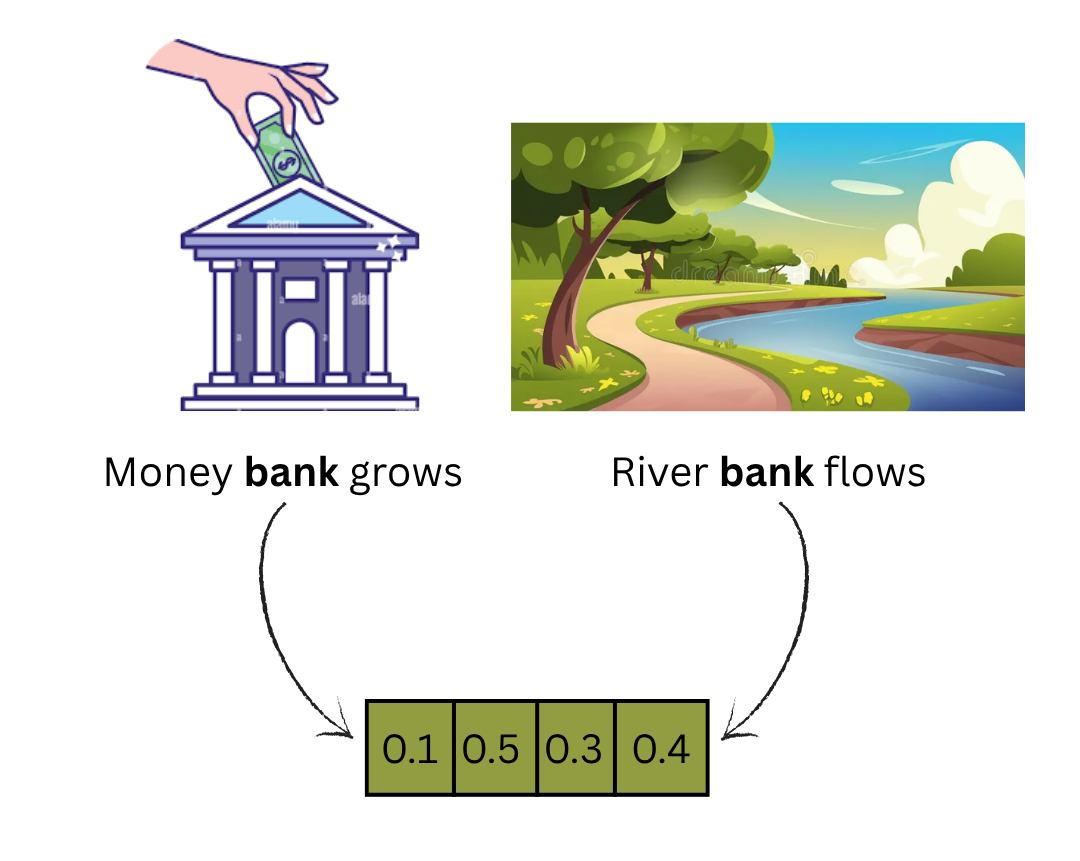
\includegraphics[width=0.5\linewidth]{Self-attention/same-word-embedding.png}
    \caption{Same word embedding of \textit{bank}}
\end{figure}

% SECTION 2: Contextual embeddings
\section{Contextual embeddings}

To solve the problem of determining context, we use \textbf{contextual embeddings}, which are generated by the \textbf{self attention} block. We will assume that we do not know anything about what self-attention is and that we are deriving this for the first time. So, let us start!

Consider the sentence mentioned previously: \textit{Money bank grows}. What does the context of a word depend on? It depends on the words that come before and after it. Using this fact, we will try to write the meaning of all the words in the sentence like this:
\begin{align}
    money &= 0.8 \times money + 0.15 \times bank + 0.05 \times grows \\
    bank &= 0.2 \times money + 0.7 \times bank + 0.1 \times grows \\
    grows &= 0.15 \times money + 0.05 \times bank + 0.8 \times grows
\end{align}

The numbers are randomly assigned, such that all of them sum to 1. The equation means that the meaning of \textit{bank} in this context depends 20\% on the meaning of \textit{money}, 70\% on the meaning of \textit{bank} and 10\% on the meaning of \textit{grows}.

Since a model does not understand human language, we have to convert each word into its corresponding \textit{word embedding}. We will also replace the numbers with variables. The equation becomes:
\begin{align}
    y_{money} &= s_{11}\,e_{money} + s_{12}\,e_{bank} + s_{13}\,e_{grows} \\
    y_{bank} &= s_{21}\,e_{money} + s_{22}\,e_{bank} + s_{23}\,e_{grows} \\
    y_{grows} &= s_{31}\,e_{money} + s_{32}\,e_{bank} + s_{33}\,e_{grows}
\end{align}

Over here, $y$ represents contextual embedding and $e$ represents static word embedding. $s_{12}$ represents the similarity score between \textit{money} and \textit{bank}, $s_{13}$ represents the similarity score between \textit{money} and \textit{grows} and so on. This can be represented by the DOT product between the \textit{embedding vectors} (2 vectors are similar, i.e., close to each other if their dot product has a higher value). Hence, we can write the equation as:
\begin{align}
    y_{money} &= [e_{money} \cdot e_{money}^T]\,e_{money}
              + [e_{money} \cdot e_{bank}^T]\,e_{bank}
              + [e_{money} \cdot e_{grows}^T]\,e_{grows} \\
    y_{bank} &= [e_{bank} \cdot e_{money}^T]\,e_{money}
             + [e_{bank} \cdot e_{bank}^T]\,e_{bank}
             + [e_{bank} \cdot e_{grows}^T]\,e_{grows} \\
    y_{grows} &= [e_{grows} \cdot e_{money}^T]\,e_{money}
              + [e_{grows} \cdot e_{bank}^T]\,e_{bank}
              + [e_{grows} \cdot e_{grows}^T]\,e_{grows}
\end{align}

For machine learning models, training is better if we provide normalized inputs. Hence, we pass all the $s_{ij}$ values through a \textit{softmax} function. A softmax function acting on input \textit{a} present in the set [a, b, c] does the following:
$$softmax(a) = \frac{e^a}{e^a + e^b + e^c}$$

We apply this individually to each of the word embeddings, Hence:
$$w_{11} = softmax(s_{11}) = \frac{e^{s_{11}}}{e^{s_{11}} + e^{s_{12}} + e^{s_{13}}}$$

Applying this to all the similarity scores, we get the output as:
\begin{align}
    y_{money} &= w_{11}\,e_{money} + w_{12}\,e_{bank} + w_{13}\,e_{grows} \\
    y_{bank} &= w_{21}\,e_{money} + w_{22}\,e_{bank} + w_{23}\,e_{grows} \\
    y_{grows} &= w_{31}\,e_{money} + w_{32}\,e_{bank} + w_{33}\,e_{grows}
\end{align}

Phew! That was a lot of math. This entire flow can be represented in a simpler manner using linear algebra. ($n$ is the dimension of the embedding vector)
\begin{figure}[H]
    \centering
    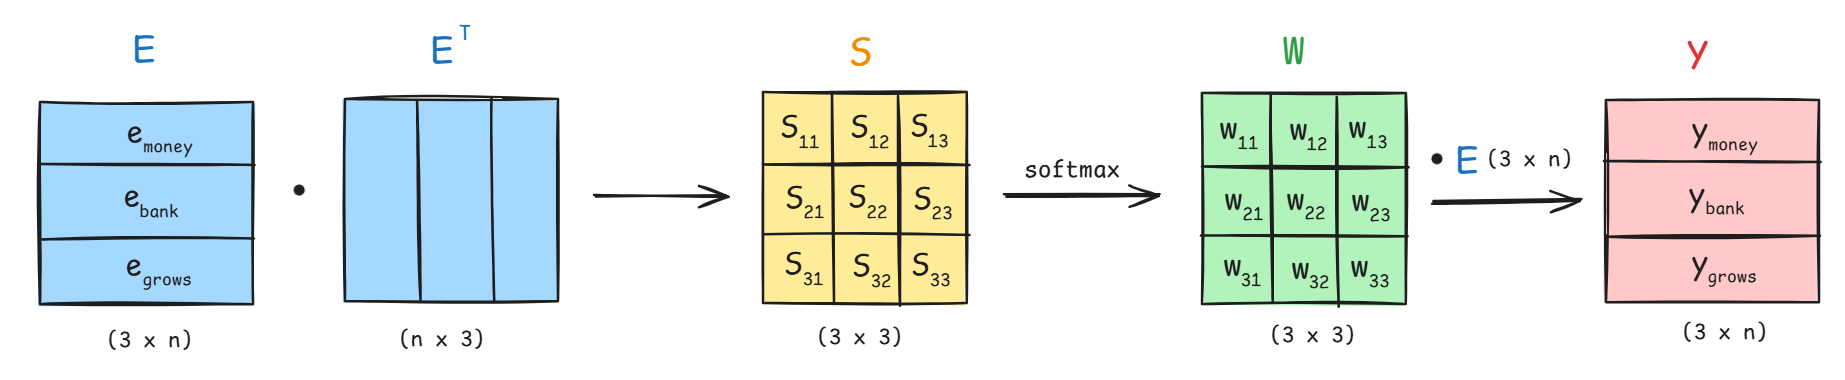
\includegraphics[width=1\linewidth]{Self-attention/contextual-embedding.png}
    \caption{Contextual embedding using linear algebra}
\end{figure}

Finally, we converted static embeddings into contextual embeddings. There are 2 things to note in this approach:
\begin{itemize}
    \item Since this method uses matrix multiplications, the embeddings of all the words can be processed simultaneously (in parallel) at the same time. This makes this process much faster than traditional methods, since parallel computations can be performed efficiently using GPUs.
    \item There are no trainable parameters in this method. This means that the contextual embeddings generated are \textit{general}. But the context of a word depends on the task that we are performing (a word may have a different context in machine translation than in text summarisation). Hence, we need to find a way to assign some parameters into this method, whose value depends on the specific task that we are performing.
\end{itemize}

% Query, key and value
\section{Query, Key and Value}

If we inspect the process a little closer, then we will find that every static embedding appears in 3 places.
\begin{figure}
    \centering
    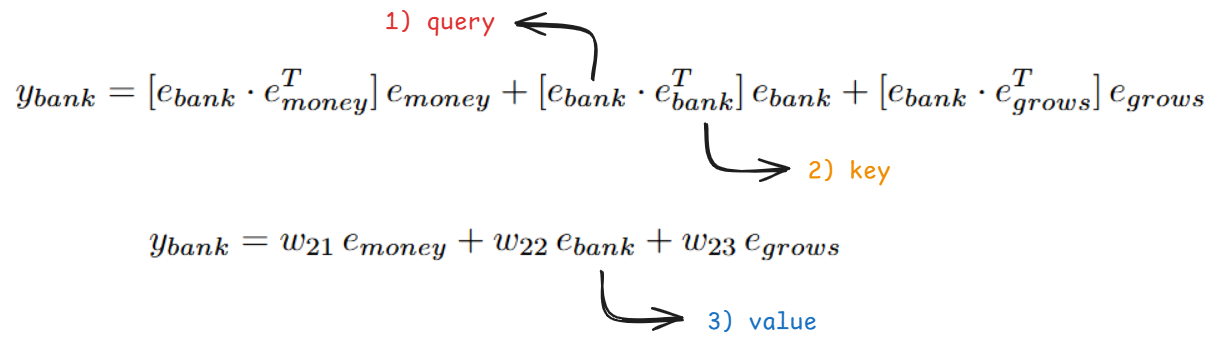
\includegraphics[width=0.5\linewidth]{Self-attention/embeddings-use.png}
\end{figure}

In the 1st place, the embedding asks what is the words' similarity with it. In the 2nd place, it answers the question. In the 3rd place, it provides a value to the contextual embedding. Hence the places are known as \textbf{query, key} and \textbf{value}.

It is not correct to use the same vector (embedding) for performing 3 different tasks. It is better to use different vectors derived from the embedding. The vectors can be derived by multiplication of the embedding vector with scalars (in which case the vectors are scaled (change in magnitude)) or matrices (which brings about a linear transformation of the vectors (change in magnitude and direction)). To keep things flexible, we use matrices. The values of the matrices are parameters (weights) that adjust their values according to the task.

Each word embedding produces 3 vectors - \textit{query, key} and \textit{value}. We need 3 matrices for generating these vectors from the \textit{embedding vector}. These matrices are called $W^Q, W^K$ and $W^V$. The entire flow can once again be represented using linear algebra.
\begin{figure}[H]
    \centering
    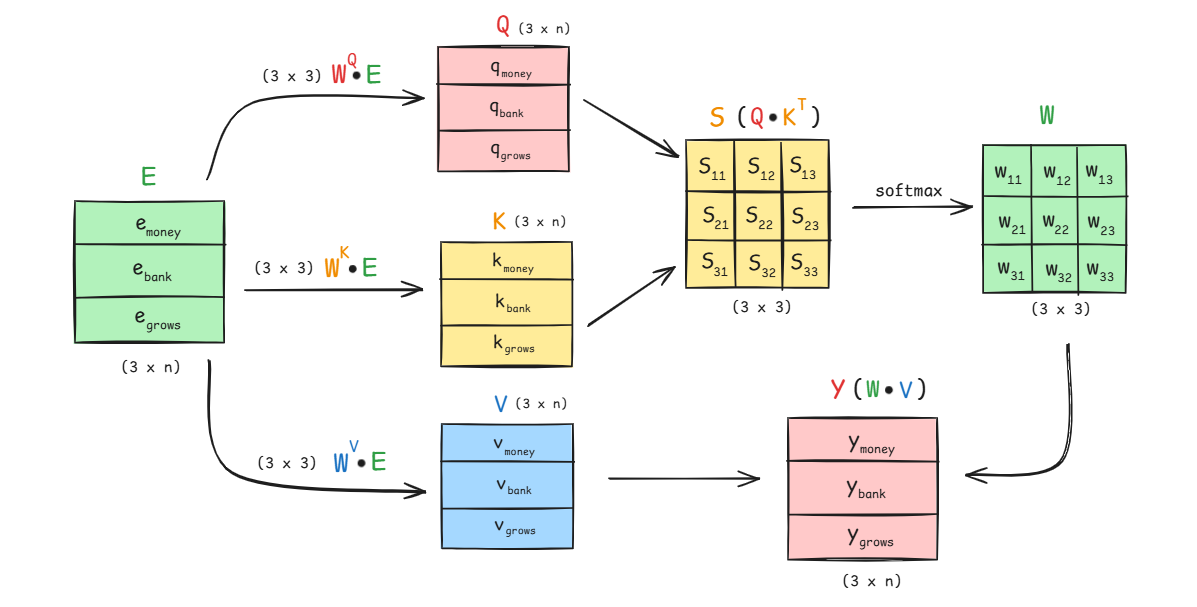
\includegraphics[width=1\linewidth]{Self-attention/self-attention.png}
    \caption{Self-attention mechanism}
\end{figure}

Thus, we generated task-specific contextual embeddings of words from static embeddings. This is the \textbf{self-attention mechanism}. A compact formula for this is:
$$Attention\,(Q, K, V) = softmax\,(QK^T)V$$

% Scaled-dot product
\section{Scaled-dot product}

The original expression for attention (as used in the paper is):
$$
Attention\,(Q, K, V) = softmax \left(\frac{QK^T}{\sqrt{d_k}}\right)V
$$

where $d_k$ is the dimension of the embedding vector. To understand why the scaling is done, we need to understand some concepts.

\subsection{Variance of dot product}

As the dimension of a vector increases, the variance associated with its dot product value (with another vector of same dimension) also increases. The following is a mathematical derivation of the same.

Let us assume that we have query and key vectors denoted by $q$ and $k$ of dimension $d$. The dot product is:
$$\textbf{q} \cdot \textbf{k} = \sum_{i=1}^{d} q_ik_i$$

We assume that both $q$ and $k$ are standardized. That is:
\begin{align}
    E[q_i] = 0, \, \, Var(q_i) = 1 \\
    E[k_i] = 0, \, \, Var(k_i) = 1
\end{align}

\begin{align}
    \therefore Var(q_i) &= E[q_i^2] - E[q_i]^2\\
    \implies E[q_i^2] &= 1
\end{align}

Same applies for $k_i \implies E[k_i^2] = 1$

Since \textbf{q} and \textbf{k} are independent of each other,
\begin{align}
    E[q_ik_i] &= E[q_i]E[k_i] = 0\\
    E[q_i^2k_i^2] &= E[q_i^2]E[k_i^2] = 1
\end{align}

Now,
$$Var(\textbf{q} \cdot \textbf{k}) = Var(\sum_{i=1}^{d} q_ik_i) = \sum_{i=1}^d Var(q_ik_i)$$

Using the equations derived above,
\begin{align}
    Var(q_ik_i) &= E[q_i^2k_i^2] - E[q_ik_i]^2 = 1\\
    \implies Var(\textbf{q} \cdot \textbf{k}) &= \sum_{i=1}^d = d
\end{align}

Hence, the variance is equal to the dimension of the vector. In order to substantiate this point, let us consider a setup. We will take a pair of vector (\textbf{q} and \textbf{k}) of a given dimension, standardise them and perform their dot product. This process is repeated 1000 times for vectors of different dimensions (10, 100, 1000). The distribution of dot product values is shown.
\begin{figure}[H]
    \centering
    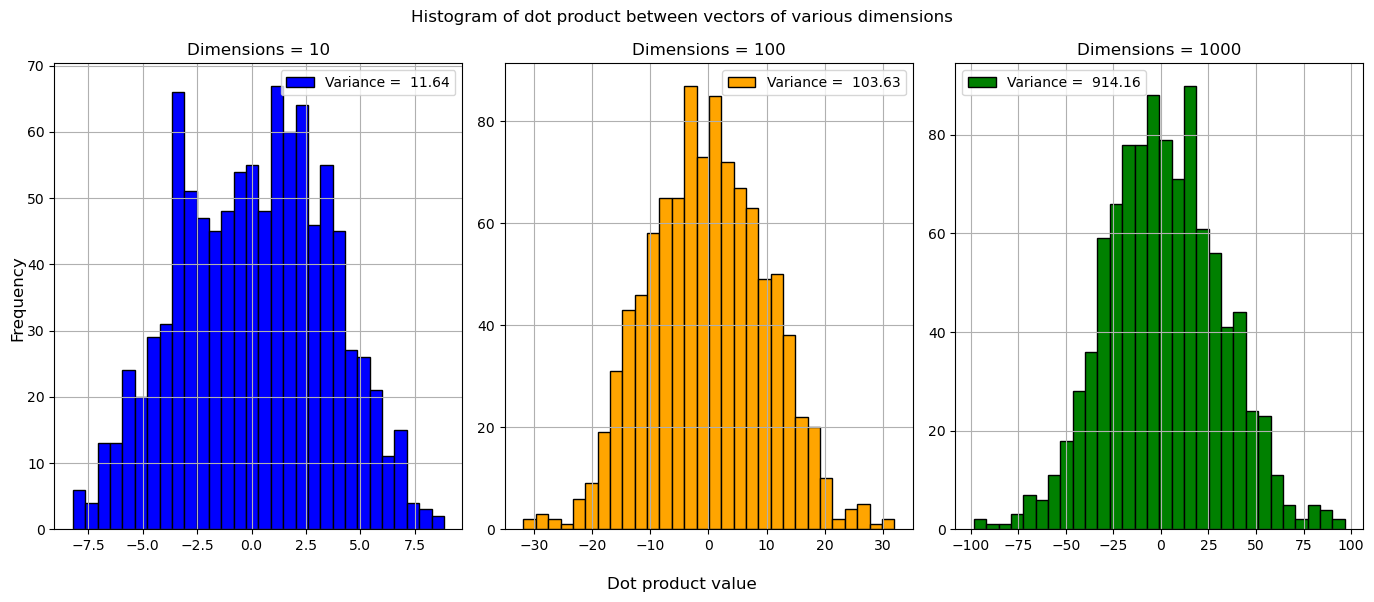
\includegraphics[width=0.8\linewidth]{Self-attention/variance-dot-product.png}
    \caption{Distribution of dot product values}
\end{figure}

As can be seen from the histogram and from the calculated values, the variance is nearly equal to the dimension of the vectors.

\subsection{Nature of softmax function}
Given below is an implementation of the softmax function on 2 lists.
\begin{figure}[H]
    \centering
    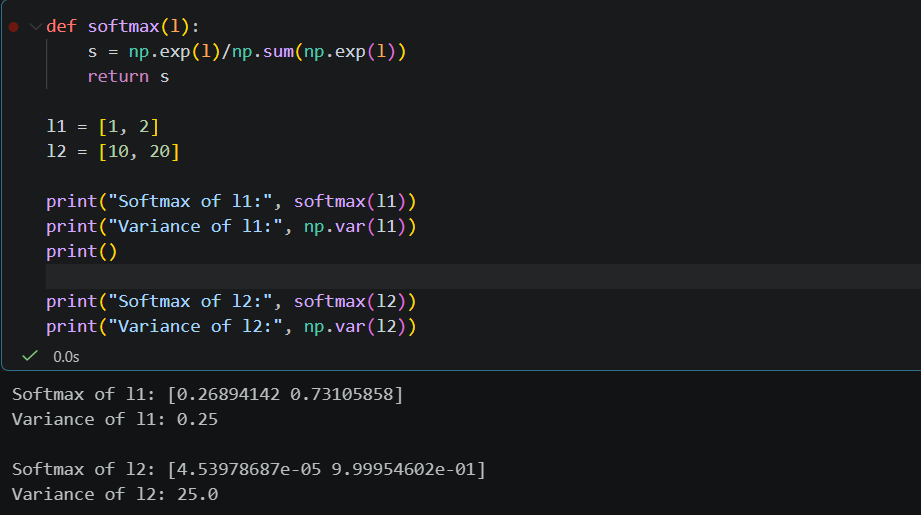
\includegraphics[width=0.5\linewidth]{Self-attention/softmax.png}
    \caption{Softmax implementation}
\end{figure}

As can be seen, softmax for a distribution having a high variance pushes the lower numbers close to 0 and higher numbers close to 1. This creates a problem. We apply the softmax function at the end to get the weight matrix $W$. If this happens for embedding vectors of higher dimensions (high variance of dot product), then some of the weight values will be close to 0, whereas some will be close to 1.

\subsection{Vanishing gradient problem}

The value of the weights is updated during the training process through backpropagation. It is an algorithm that minimizes the loss between actual and predicted values using the gradient descent algorithm. The expression for gradient descent is as follows:
$$w_i^n = w_i - \eta \frac{\partial L}{\partial w_i}$$

$w_i$ - current value of the weight\\
$w_i^n$ - updated value\\
$L$ - loss\\
$\eta$ - learning rate

Let the softmax function be represented as $\sigma_i$. Loss does not depend directly on $w_i$. For calculating $\frac{\partial L}{\partial w_i}$ (gradient), we need to calculate $\frac{\partial \sigma_i}{\partial w_i}$ (chain rule). Now consider the derivative of the softmax function:

\[
\frac{\partial \sigma_i}{\partial z_i}
=
\sigma_i(1-\sigma_i).
\]

When \(\sigma_i\) is close to \(0\) or \(1\),

\[
\sigma_i(1-\sigma_i)\approx 0.
\]

Therefore the gradient flowing through the softmax becomes very small. This is known as the \textbf{vanishing gradient problem}.

As a result:
\begin{itemize}
    \item The value of the weights is not updated.
    \item Weights near \(0\) receive almost no learning signal.
    \item Weights near \(1\) are nearly saturated.
    \item Training becomes slow and unstable.
\end{itemize}


For solving the following issues, it is necessary that the variance of dot product remains constant even if the dimension of the vectors increases. The variance of a distribution scales as follows:
$$Var(q_i) = a \implies Var(cq_i) = c^2a$$

Hence, to keep the variance constant, we must divide by some factor. In our case, since variance scales as the dimension of the vectors, we divide by $\sqrt{d_k}$ to keep the variance constant. That is why we scale the dot-product.

\textbf{NOTE}: All of the graphs and code given above are available in this \underline{\href{https://colab.research.google.com/drive/1N-T9v-Fbj2sj9hBlTvLmCdg0MTnMip0Q?usp=sharing}{notebook}}

% Multi-head attention
\section{Multi-head attention}

Consider the following sentence: \textit{The man saw the astronomer with a telescope}. This can have 2 meanings:
\begin{itemize}
    \item The man used a telescope to see the astronomer
    \item The man saw that the astronomer was carrying a telescope.
\end{itemize}

Depending on the context of the text, either one of them will be true. Unfortunately, self-attention can capture only 1 meaning. Hence, we use multiple self-attention blocks together to capture different meanings of ambiguous sentences. This is called \textbf{multi-head attention}.
\begin{figure}[H]
    \centering
    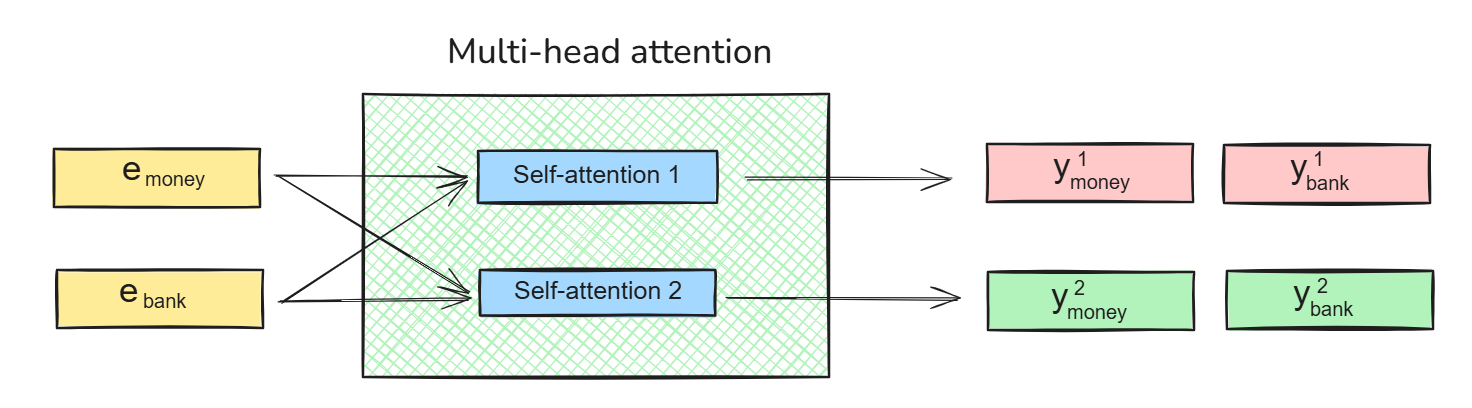
\includegraphics[width=1\linewidth]{Self-attention/multi-head-attention.png}
    \caption{Mutlti-head attention}
\end{figure}

The entire flow is provided below. Over here, after the matrices $Y_1$ and $Y_2$ are generated, they are stacked horizontally (side-by-side) and multiplied by $w_0$ to give the final output. The values of the matrix $w_0$ are calculated during the training process.
\begin{figure}[H]
    \centering
    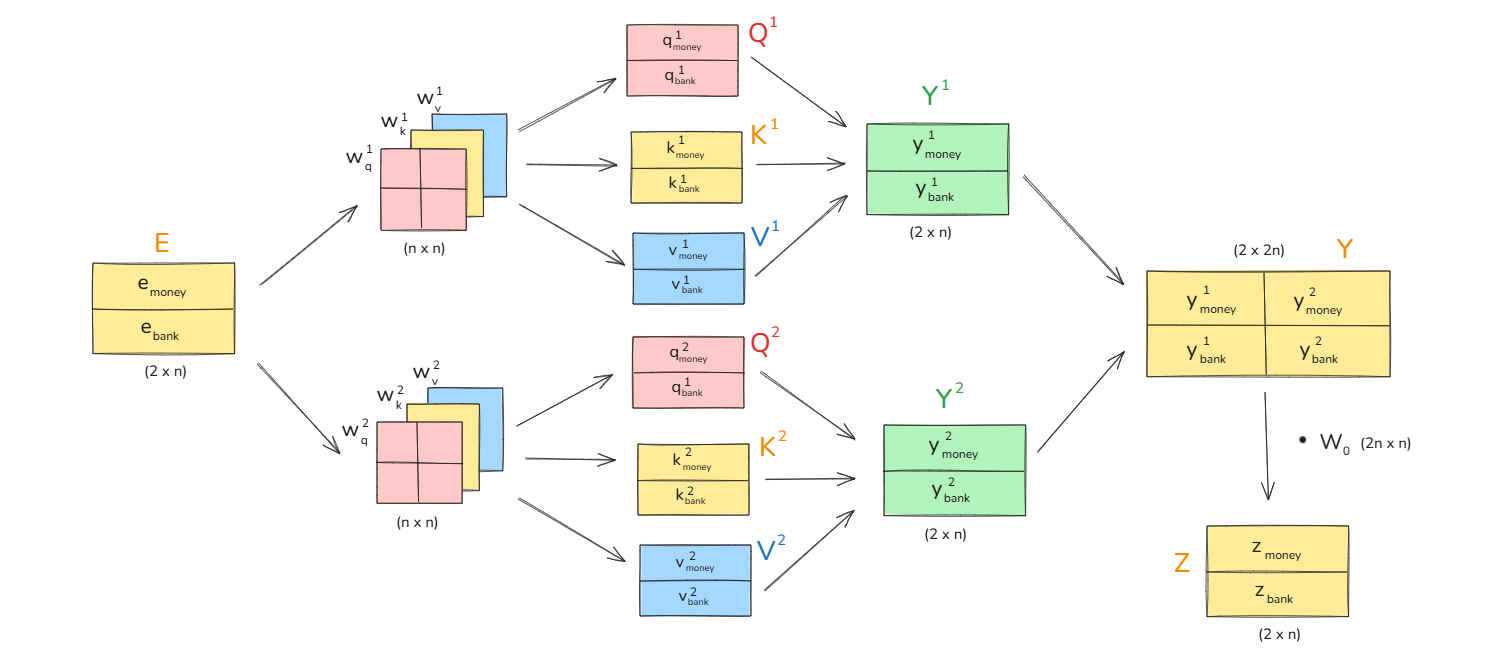
\includegraphics[width=1\linewidth]{Self-attention/multi-head-attention-algbra.png}
    \caption{Multi-head attention flow using linear algebra}
\end{figure}